%\documentclass[sigconf, titlepage, twoside]{acmart}
\documentclass[12pt,titlepage, twoside]{article}
%\usepackage{titlesec}

% language stuff
\usepackage{german}           % deutsche Überschriften etc.
\usepackage[utf8]{inputenc} % direkte Einbgabe von Umlauten

% Layout-Einstellungen
\usepackage{parskip}          % Abstand statt Einrückung
\frenchspacing                % no extra space after periods
\usepackage{parskip}          % paragraph gaps instead of indentation
\usepackage{times}            % default font Times
\tolerance=9000               % avoid words across right border

% miscellaneous
\usepackage{graphicx}         % graphics
\usepackage{hhline}           % double lines in tables
\usepackage{amsfonts}         % real numbers etc.
\usepackage[rightcaption]{sidecap} % figure captions on the right (optional)
\usepackage{hyperref}         % for URLs
\usepackage{listings}         % for code samples
\usepackage{fancyhdr}         % for header line
\usepackage{lastpage}         % for last page count

% Hier bei Bedarf die Seitenränder einstellen
\usepackage{geometry}
%\geometry{a4paper}
\geometry{a4paper,left=25mm,right=25mm, top=3.5cm, bottom=2.5cm} 

% Kopf- und Fußzeile
\fancyhead{} % clear all header fields
\fancyhead[RO,LE]{\leftmark}

%%%%%%%%%%%%%%%%%%%%%%%%%%%%%%%%%%%%%%%%%%%%%%%%%%%%%%%%%%%%%%
\begin{document}


%-------------------------------------------------------------
\begin{titlepage}
%-------------------------------------------------------------
\begin{center}
{\Large\bf Analyse von Pflanzenwachstum auf Basis von 3D-Punkwolken}\\[3cm]

{\bf Masterarbeit}\\
zur Erlangung des Grades {\em Master of Science}\\[1.5cm]

an der\\
Hochschule Niederrhein\\
Fachbereich Elektrotechnik und Informatik\\
Studiengang {\em Informatik}\\[3cm]

vorgelegt von\\
Jakob Görner\\
1003660\\[3cm]
Datum: \today\\[3cm]

Prüfer: Prof.~Dr.~Regina Pohle-Fröhlich\\
Zweitprüfer: Prof.~Dr.~Christoph Dalitz

\end{center}
\end{titlepage}

\pagestyle{empty}
\cleardoublepage

\newpage


%-------------------------------------------------------------
\section*{Eidesstattliche Erklärung}
%-------------------------------------------------------------
\begin{tabbing}
Name: \hspace{4em}\= Jakob Görner\\
Matrikelnr.: \> 1003660\\
Titel: \> Analyse von Pflanzenwachstum auf Basis von 3D-Punkwolken
\end{tabbing}

Ich versichere durch meine Unterschrift, dass die vorliegende
Arbeit ausschließlich von mir verfasst wurde.
Es wurden keine anderen als die von mir angegebenen Quellen und Hilfsmittel
benutzt.

Die Arbeit besteht aus \pageref{LastPage} Seiten.

\vspace{8ex}
\begin{tabbing}
\underline{\hspace{14em}} \hspace{3em}\= \underline{\hspace{14em}} \\
Mönchengladbach, \today \> Unterschrift
\end{tabbing}

\newpage
%\begin{abstract}
%-------------------------------------------------------------
\section*{Zusammenfassung}
%-------------------------------------------------------------
In dieser Arbeit soll eine Anwendung zum Analysieren von Pflanzen-Wachstum und weiteren Merkmalen des Wachstumsprozesses einer Pflanze erstellt werden. Es soll aus einer Reihe Bilder einer Pflanze, die mit einer gängigen Smartphone-Kamera aufgenommen sind, eine Punkwolke erzeugt werden. 
Aus der Punktwolke sollen die Punkte die zur Pflanze gehören extrahiert werden um diese weiter zu analysieren. Die extrahierten Punkte werden zur weiteren Analyse in Stamm und Blatt Punkte segmentiert, die dann weiter analysiert werden können.
Des weiteren sollen Werte wie das Wachstum der Pflanze ermittelt werden. Hierzu müssen mehrere Punktwolken über Zeit miteinander verglichen werden.
Die Anwendung soll mit möglichst wenig Bildern auskommen um den Datentransfer zu minimieren.

\setcounter{page}{1}
%-------------------------------------------------------------
\section*{Abstract}
%-------------------------------------------------------------
Development of an application made to analyse plant growth over time and further characteristics of a plant represented as a point cloud. The point cloud should be generated out of a set of images of the plant, taken with a common smartphone.
The point cloud should be splitted in leave and stem points to count leaves and analyse the stem further. Also other characteristics as the hight should be analysed. For this reason multiple point clouds has to be analysed over time.
The application should need as few pictures as possible to reduce the amount of transfared data.

%\end{abstract}
\newpage

\pagestyle{plain}
\tableofcontents
\newpage

%-------------------------------------------------------------
% default a), b), c) numbering
\renewcommand{\labelenumi}{\alph{enumi})} 

%=============================================================


\section{Motivation}
%-------------------------------------------------------------
\label{sec:einleitung}
Diese Arbeit wird im Rahmen eines Projekts mit der Universität xx durchgeführt. Im Rahmen dieser Arbeit soll eine Anwendung entstehen, die in Uganda zum Einsatz kommen soll.
Die Anwendung soll mit nicht invasiven Methoden zur Unterstützung bei der selektiven Züchtung eingesetzt werden.
Ziel ist es eine Software zu schaffen die es ermöglicht aus Bildern von Pflanzen 3D Punktwolken(Punktwolken) zu generieren und diese zu analysieren.
Es soll mit der zu entwickelnden Anwendung möglich sein Aussagen über das Wachstum über Zeit, die Entwicklung der Blätter und der Stämme zu treffen. 
Mit diesen Daten sind Analysen möglich die auf das Wachstum einer Pflanze unter bestimmten Bedingungen schließen lassen.
Hierbei sind besondere Anforderungen an den Prozess der Datengewinnung und Übertragung, dass zum einem der Betrieb kostengünstig ist - das betrifft insbesondere den Endverbraucher, der möglichst wenig Datenmengen an den Server, der die Rechenkapazität bereit stellt übertragen muss.
Desweiteren muss die Datengewinnung mit einem Mobiltelefon oder einer anderen Kamera möglich sein.Spezielle Aufnahmegeräte wie ein LIDAR-Scanner sollten nicht nötig sein.


\newpage
\section{Stand der Technik}
%-------------------------------------------------------------
\label{sec:stand}
%Hier müssen Sie beschreiben wie die Situation vor Ihrem Beitrag war.
%Dazu gehören die Vorarbeiten anderer, auf denen Sie aufsetzen, die
%bisher eingesetzte Software oder Hardware und allgemeine
%bekannte Techniken, die in Ihrer Arbeit zum Einsatz kamen.
%
%In diesen Abschnitt gehören alle Aspekte, die zum Verständnis der
%Arbeit erforderlich sind, aber einem mit der Aufgabenstellugn nicht vertrauten
%fachkundigen Leser nicht zwangsweise bekannt sind.

Drei Kernprobleme müssen betrachtet werden. Zuerst muss aus einer Menge an Bilder eine Punkwolke generiert werden. Danach muss die Punktwolke Segmentiert werden um den Hintergrund zu entfernen und die einzelnen Teile der Pflanze weiter zu analysieren. 
Zuletzt müssen zwei Punktwolken einer Pflanze zu verschiedenen Zeitpunkten miteinander registriert werden um Aussagen über das Wachstum einer Pflanze treffen zu können.

\subsection{Generierung einer 3D Punkwolke aus Bildern}
\label{sec:stand:pointcloud}

Generell kann man zwischen zwei Methoden der Generierung von Punktwolken unterscheiden, die jeweils verschiedene Verfahren beziehungsweise Techniken anwenden.

Die erste Methode nutzt Hardware wie LIDAR-Scanner \cite{lidar} um Punkwolken direkt zu erzeugen. Es gibt eine Reihe von Sensoren die das ermöglichen. Da der Großteil der Sensoren aus kostengrünen nicht in Frage kommt sei hier nur noch der RGB-D erwähnt. 
Dieser liefert neben den Farbwerten für ein Bild auch noch eine Tiefeninformation für jeden Pixel. In einigen Smartphone-Modellen wird bereits ein solcher Sensor verbaut.

Die andere Methode ist die Photgeometrie, bei der die Punktwolke aus Bildern, einer Szene aus verschiedenen Perspektiven, generiert wird. Eine der bekanntesten Algorithmen ist SIFT \cite{Sift3D}.
Einige Verfahren benötigen genaue Informationen über die Kamera Position, Ausrichtung und andere Angaben wie die Brennweite der Linse etc. andere wiederrum lesen diese Informationen aus den Bildern direkt aus oder schätzen diese \cite{ODM}.

Es wurden in den letzten Jahren große Fortschritte im Bereich Deep Learning auf 3D-Punkwolken gemacht, zur Gewinnung von 3D-Punkwolken.

%TODO Verfahren auflisten SIFT, RANSAC?, 

\subsection{Segmentierung von 3D Punkwolken}
\label{sec:stand:segmentierung}

Bei der Analyse von Pflanzen in Form von 3D Punktwolken gibt es einige nicht gelernte Lösungen \cite{ThreeBasics} \cite{RegionGrowing} die das segmentieren von 3D Punktwolken von Pflanzen in Stiele und Blätter behandeln, viele dieser Ansätze haben aber das Problem, dass sie nur unter Laborbedingungen gute Ergebnisse liefern. 
Insbesondere die hohe Qualität der Punktwolken die meist mit einem LIDAR-Scanner oder einem vergleichbaren Gerät erzielt wird, kann mit bildbasierten Methoden nicht oder nur mit sehr großen Datenmengen erreicht werden. 
Ein weiteres Problem das viele Lösungen haben ist, dass der Hintergrund manuell entfernt wird und erst auf der freigestellten Pflanze der eigentliche Ansatz ausgeführt wird. 
Um diese Lösungen dennoch in einer voll automatischen Pipeline nutzen zu können muss das freistellen der Pflanzen erst automatisiert werden.
Auch im Bereich Segmentierung wurden große Fortschritte im Bereich Deep Learning auf 3D-Punkwolken gemacht, die mit einer angelernten Netzarchitektur bestimmte Objekte erkennen und Teile davon segmentieren. Diese Ansätze können auch auf Pflanzen angewandt werden. Dazu müssen Architekturen wie PointNet\cite{qi2017pointnet}/PointNet++\cite{qi2017pointnet++} auf Punktwolken von Pflanzen trainiert werden.  

\subsection{Registrierung von 3D Punkwolken}
\label{sec:stand:registrierung}

Die am weiten verbreitete Method zur Registrierung von 3D Punktwolken ist Iterative Closest Points (ICP). ICP basiert auf dem Ansatz das zwei Punktwolken iterativ aneinander angenähert werden und bei jeder Iteration der Abstand minimiert wird.
Die meisten Implementierungen von ICP beachten aber nicht die Skalierung der Punktwolken. Es gibt einige wenige Ansätze für dieses Problem. 
Ein weiteres Problem bei ICP ist, dass es in lokalen Minima Lösungen finden kann. Daher muss eine gute Initiale Transformation gefunden werden. Dieses Problem kann durch globale ICP gelöst werden. Hierbei wird der zu durchsuchend Suchraum SO(3) mittels Branch \& Bound Verfahren durchsucht.
Auch für das Registrierung-Problem gibt es Lösungen die auf Neuronal Netzen basieren, aber auch hier gibt es das Problem, dass es nur wenige Ansätze gibt die mit Skalierung umgehen können.

\newpage
\section{Realisierung}
%-------------------------------------------------------------
\label{sec:realisierung}
Es müssen vier Teilprobleme berücksichtigt werden. Zu Beginn muss aus einer Reihe Bilder eine Punktwolke generiert werden. Hauptziel hierbei ist es möglichst wenig Bilder zu benötigen. 
Trotzdem müssen Aspekte wie die Qualität der Punkwolken berücksichtigt werden. 

Ein zweites Problem ist die Registrierung zweier Punktwolken einer Pflanze zu verschiedenen Zeitpunkten um diese Vergleichen zu können. 
Hierbei gilt es die ideale Transformation $T$ bestehend aus Rotation, Skalierung und Translation zu finden um die beiden Punktwolken so realitätsnah wie möglich aneinander aus zu richten.
Es werden drei Ansätze überprüft dieses Problem zu lösen. 
Der erste Ansatz basiert auf der Idee, beim Beginn einer neuen Zeitserie zur Analyse eines Wachstumsprozesses, eine Punktwolke des Hintergrunds zu erstellen und die Punktwolken der einzelnen Zeitpunkte mit diesem Hintegrund zu registrieren. So wird ein Verhältnis geschaffen das dem der realität entspricht.
Der zweite Ansatz basiert darauf das die Registrierung direkt zwischen zwei Zeitpunkten erfolgt. Hierbei kann es zu Abweichungen von der Realität kommen, wenn die Pflanzen skaliert werden müssen für die Registrierung.
Der letzte Ansatz soll überprüfen ob es mittels eines platziertem Objekts möglich ist die skalierung der Punktwolke zu ermitteln und so das Problem beim direkten Vergleich zweier Szenen lösen soll.

Das dritte Problem ist die Segmentierung der Punktwolke in Stamm, Blätter und Hintergrund. Hier gibt es viele Ansätze dieses Problem zu lösen. Allerdings ist es schwer eine allgemein gültigen Lösung zu finden. 
Ziel ist es daher eine Lösung zu finden die auf möglichst vielen Varianten von Pflanzen funktioniert. 
Das Problem der Segmentierung ist essentiell für die weitere Analyse einer Zeitserien. Ohne die Information welche Punkte zu Stamm und Blättern gehören kann nicht auf die Entwicklung von Blättern und Stielen geschlossen werden.

Zuletzt müssen aus die bisherigen Problemen in geeignete Pipelines zusammengefasst werden und durch einen Server angesteuert werden. Hier muss die Lastverteilung und Datenhaltung beachtet werden.

\subsection{Architektur}
%-------------------------------------------------------------
\label{sec:realisierung:architektur}
%Zwingend erforderlich ist ein Überblick über die Komponenten Ihrer Lösung
%und deren Zusammenspiel. Dazu gehört in der Regel auch ein Diagramm
%der Systemarchitektur.

Die Anwendung soll über eine REST-API angesteuert werden können. Es soll möglich sein eine neue Messreihe anzulegen. Dazu müssen die Bilder für die initiale Punkwolke auf den Server übertragen werden. 
Es soll möglich sein weitere Messpunkte zu einer Messreihe hinzuzufügen. Zu einer Messreihe sollen Auswertungen zur Verfügung gestellt werden. 
Zu jeder Messreihe soll ein Bearbeitungs-Status abgerufen werden können, da die einzelnen Pipelines asynchrone im Hintergrund ausgeführt werden sollen. 

\subsection{Umsetzung Generierung einer 3D Punktwolke aus Bildern}
%-------------------------------------------------------------
\label{sec:realisierung:implementierung1}
%Dies ist in der Regel nicht nur ein Abschnitt, sondern mehrere Abschnitte
%mit Ihrem Projekt angemessenen Überschriften. Hierhin gehört {\em nicht}
%der Sourcecode Ihrer Lösung, sondern eine textuelle und grafische
%(z.B.~Klassendiagramm) Beschreibung. Bei Quellcode beschränken Sie Sich
%bitte auf kurze, aussagekräftige Ausschnitte.

Die aus der Analyse der verschiedenen Verfahren (siehe Evaluation) ausgewählte Anwendung ODM wird als Docker bereit gestellt. Um den Docker aus zu führen muss eine Ordner-Struktur erstellt werden.
In dieser Ordner-Struktur muss ein Ordner "images" enthalten sein, der die Bilder des Datensatzes, aus dem eine Punktwolke generiert werden soll, enthält.

Ist das Verzeichnis angelegt kann der Docker gestartet werden. Hierbei muss allerdings beachtet werden, dass der Docker mit den selben Rechten wie der User arbeitet. Ansonsten werden per Standarteinstellung Root-Rechte genutzt.
Das führt dazu das auf die erstellten Daten kein Zugriff mehr existiert, was das Aufräumen erschwert.

\subsection{Umsetzung Registrierung zweier Punktwolken}
%-------------------------------------------------------------
\label{sec:realisierung:implementierung2}

Es wurden mehrere Verfahren und Implementierungen mit einander verglichen. Es wurde versucht ein Pipeline zu erstellen die eine gute Initiale Lösung findet ohne den ganzen Suchraum SO(3) zu durchsuchen.
Die Pipeline sucht nach einer Ebene in der Punkwolke und richtet die Punkwolke so aus, dass die Ebene auf der Ebene liegt, die die x und y Achse bilden. Danach werden einige wiederholte ICP Schritte und andere Registrierungsmethoden angewandt.

Ein weiterer Ansatz war es DCP so abzuwandeln das statt Translations-Vektor und Rotations-Matrix direkt die ganze Transformations-Matrix geschätzt wird. Dazu muss nur SVD-Head angepasst werden 
und bei der Eingabe eine weitere Dimension hinzugefügt werden. Wenn man nun die Singulärwert-Zerlegung von H das nun 4x4 groß ist also die richtige Dimension hat weg lässt, kann man H als schätzung für die Transformation interpretieren.

Eine weitere Version die ICP nutzt ist es einen gewissen Bereich an Skalierungen zu durchlaufen und für jede Skalierung werden die beiden Punktwolken via ICP miteinander registriert.
Wurden alle Skalierungen getestet wird die mit dem besten Ergebnis übernommen.

\subsection{Umsetzung Segmentierung}
%-------------------------------------------------------------
\label{sec:realisierung:implementierung3}

Zur Segmentierung der Pflanzen-Punktwolke in Stamm und Blätter wurde ein Ansatz verfolgt der an den in \cite{ThreeBasics} angelehnt ist, der mittels der Hauptkrümmung eines Punktes ermitteln soll ob es sich um ein Blatt oder einen Stiel handelt. 
Hierbei wird eine einfache Entscheidungsregel $f(x)$ mittels eines Schwellwerts $T_k$ genutzt: Ist die Stärke der Krümmung $k(x)$ des Punktes höher als der Schwellwert handelt es sich um einen Stiel da diese einen größere Krümmung haben als Blätter.
Die Schwierigkeit ist es einen guten Schwellwert und eine gute Kennzahl für die Stärke der Krümmung zu finden.

Die Hauptkrümmung eines Punktes $p_i$ kann über die Normalen des Punktes und der $k$ nächsten Nachbarpunkte $P_i$ berechnet werden.

\begin{equation}
\label{eq:hauptkruemmung:1}
\vec{m}_j = (I - \vec{n}_i \otimes \vec{n}_i ) \cdot \vec{n}_j
\end{equation}

Aus den Abbildungen $\vec{m}_j$ für alle $P_i$ kann die Kovarianzmatrix $C_i$ berechnet werden.

\begin{equation}
\label{eq:hauptkruemmung:2}
C_i = \frac{1}{k} \sum_{j=1}^k{(\vec{m}_j - \vec{\bar{m}}) \otimes (\vec{m}_j - \vec{\bar{m}})}
\end{equation}

Die Hauptkrümmung kann aus den Eigenwerten $0 \leq \lambda_1 \leq \lambda_2 \leq \lambda_3$ von $C_i$ bestimmt werden. $\lambda_3$ ist die stärkste Krümmung und $\lambda_2$ die schwächste Krümmung.

Einige untersuchte Ansätze für eine Funktion $k(p_i)$ sind in \ref{eq:hauptkruemmung:3} zu finden. 

\begin{equation}
\label{eq:hauptkruemmung:3}
\begin{array}{ll}
k_1(p_i) = \lambda_3 \\
k_2(p_i) = \lambda_2 \\
k_3(p_i) = (\lambda_3 + \lambda_2) / 2 
\end{array}{}
\end{equation}

Je höher der Wert der Funktion $f(p_i)$ aus \ref{eq:manuell_classifier} ist desto Wahrscheinlicher gehört ein Punkt zum Stiel einer Pflanze. Ein guter Wert für den Schwellwert $T_k$ muss in Experimenten für die Funktionen $k_1$, $k_2$ und $k_3$ gefunden werden.

\begin{equation}
\label{eq:manuell_classifier}
f(p_i) = \left\{
\begin{array}{ll}
1 & k(p_i) \geq T_k \\
0 & \, \textrm{sonst} \\
\end{array}
\right. 
\end{equation}

In einem weiteren Ansatz wurde eine Implementierung von PointNet auf einem Datensatz von Pflanzen-Punktwolken trainiert um so einen geeigneten Classifier zu trainieren. 
Der Classifier soll für jeden Punkt einer Punktwolke bestehend aus Position und Normalen eine Schätzung liefern was der Punkt repräsentiert. Mögliche Repräsentationen können Stamm, Blatt oder Hintergrund sein.
Weitere denkbare Repräsentationen können die Früchte und Blüten der Pflanzen sein. Wird die Farbe der Punkwolke mit einbezogen, können auch Krankheitsbilder wie vertrocknende Blätter in die Repräsentation eingeschlossen werden.  
Da die Ergebnisse für PointNet nicht gut genug waren wurde eine verbesserte Version PointNet++ auf dem Datensatz trainiert. Diese wurde mit und ohne Normalen, mit 2 Labelen ohne Hintergrund und mit 3 Labeln mit Hintergrund trainiert.

Nach der Segmentierung wird das Ergebnis noch einmal überarbeitet. Für jedem Punkt $i$ werden die Schätzungen $N_i$ der $k$ ($k=10$) nächsten Nachbarn bestimmt und aus deren Repräsentationens-Schätzungen ein Histogramm $H_i$ erzeugt. 
Die Schätzung mit dem höchsten Histogramm-Wert wird als neue Schätzung $s_i$ für den Punkt genutzt \ref{eq:improve_score}. Dieser Vorgang wird für alle Punkte solange wiederholt bis es bei den Punkten zu keinen Änderungen mehr kommt oder eine maximale Itartions-Obergrenze erreicht wurde.

\begin{equation}
\label{eq:improve_score}
\begin{array}{l}
L =  \{0,1,2\}\\
w(x) = \left\{
\begin{array}{ll}
0,5 & x = 2 \\
1 & \, \textrm{sonst} 
\end{array}
\right.\\ 
H_i(x) = \sum_{j=0}^{k}{(w(x) | N_{ij} = x)}\\
x \in L\\
s_i = argmax_x(H_i(x))
\end{array}
\end{equation}

\subsection{Umsetzung Pipelines und Server}
%-------------------------------------------------------------
\label{sec:realisierung:implementierung4}

Der Server ist mit dem Python-Framework Flask erstellt. Flask bietet eine Schlanke API um neue Endpunkte zu erstellen und Daten vom Client anzunehmen. 

Ein Hintergrund-Prozess führt die einzelnen Jobs aus und sorgt für den Lastausgleich. Die Anfragen an den Server werden asynchron verarbeitet. Jede Anfrage wird in die Job-Queue eingeordnet. Diese wird vom Hintergrund-Prozess abgearbeitet.
Einzige Ausnahme bildet hier das Speichern der Bilder. Die Bilder müssen synchrone zum Request auf der Platte persistiert werden, da Flask die Datei-Streams nach dem Lebenszyklus eines Requests schließt.

Neben dem Hintergrund-Prozess wird auch der aktuelle Stand der Datenhaltung eingelesen und der Status des Servers aufgebaut. Des weiteren werden zwei Instanzen von PointNet++ gestartet. 
Eine für die Hintergrundsegmentierung und einer für die Blatt/Stiel-Erkennung.

\newpage
\section{Ergebnisse}
%-------------------------------------------------------------
\label{sec:ergebnisse}
%Hierhin gehört eine Beschreibung der von Ihnen durchgeführten Tests zur
%Verifikation bzw.~Qualitätssicherung Ihrer Lösung. Wenn Sie Messungen
%durchgeführt haben, so stellen Sie die Ergebnisse hier in Tabellen und
%Diagrammen dar.
%
%Auch die Diskussion der Messergebnisse oder der Besonderheiten der
%Testergebnisse gehört hierher.

\subsection{Vergleich von Verfahren zur Generierung von 3D-Punktwolken auf Basis von Bildern}

Um eine geeignete Software zur Generierung von 3D-Punktwolken auszuwählen muss erst entschieden werden nach welchen Gütekriterien verschiedene Anwendungen betrachtet werden sollen und wie wichtig diese sind.
Bei dieser Arbeit ist die nötige Anzahl der Bilder die zur Generierung einer Punktwolke mit genug Information nötig sind das wichtigste Kriterium. 
Um dieses Kriterium zu messen muss ein Goldstandart von der fotografierten Szene als 3D-Punktwolke erstellt werden, mit dem Verglichen werden kann.
Dieser Goldstandart kann erstellt werden, indem alle Fotografien genutzt werden die zur Verfügung stehen und damit alle Verfahren eine Punktwolke erstellen zu lassen. 
Unter den erstellten Punktwolken kann die ausgesucht werden die die Szene am besten repräsentiert. 
Das trifft auf die Punkwolke zu die den höchsten Detail-Grad hat und möglichst wenig Fehler, wie fehlende Teile der Szene oder Rauschen enthält.
Die so erstellte Szene sollte nachbearbeitet werden um etwaige Fehler wie Rauschen manuell zu entfernen.
Weitere Maße um die Güte des Goldstandarts zu bewerten ist die Anzahl der Punkte in der Wolke oder die Dichte der Punkte in der normalisierten Punktwolke.

Nun kann mit weniger Bildern aus dem selben Datensatz ein weitere Punktwolke generiert werden und die Distanz der Punkte der Goldstandart-Punktwolke zum jeweils nächsten Punkt der erstellten Punktwolke gemessen werden.
Die Summe dieser Abstände kann als Fehlermaß genutzt werden. Bei der Berechnung der Abstände muss beachtet werden, dass die Punkwolken mit dem Goldstandart registriert ist.

Ein weiterer Punkt bei der Bewertung des Verfahrens zur Generierung von 3D Punktwolken ist die Zeit die benötigt wird die Punkwolke zu generieren.

\subsection{Vergleich von Verfahren zur Registrierung 3D-Punkwolken}

Vergleich DCP /  PointNetLK

Verleich NN / ICP

\subsection{Vergleich von Verfahren zur Segmentierung von Pflanzen auf 3D-Punkwolken}

Als Datenbasis wurden 144 handgelabelte Punkwolken von verschiedenen Pflanzen gewählt. Darunter sind Tomaten, Mais, Paprika, Avocado, Bananen und weitere nicht bekannte Sorten. 
Da diese Datenbasis für das Training eines Neuronalen Netz recht klein ist wurde aus jeder einzelnen Punktwolke bis zu 20 Subsample erstellt. Diese wurden so erstellt, dass zufällig $n$ Punkte aus einer Punktwolke gezogen und entfernt wurden.
Des weiteren sind die Daten so aufbereitet das der Boden der Punktwolke an der XY-Ebene ausgerichtet ist und der Stiel bei geradem Wachstum richtung z-Achse zeigt. Des weiteren sind die Punkte in der Punktwolke auf 1 normiert. 
Das heißt sie liegen in dem quadratischen Raum den die beiden Punkte $(0,0,0)$ und $(1,1,1)$ aufspannen. Die Daten werden in einem Verhältnis 80 zu 10 zu 10 in Trainings-, Test- und Evaluations-Datensatz aufgeteilt.

Vergleich Training mit/ohne Hintergrund
    Mit Hintergrund -> lohnt es sich nur das Zentrum zu betrachten?

\begin{figure}
    \centering
        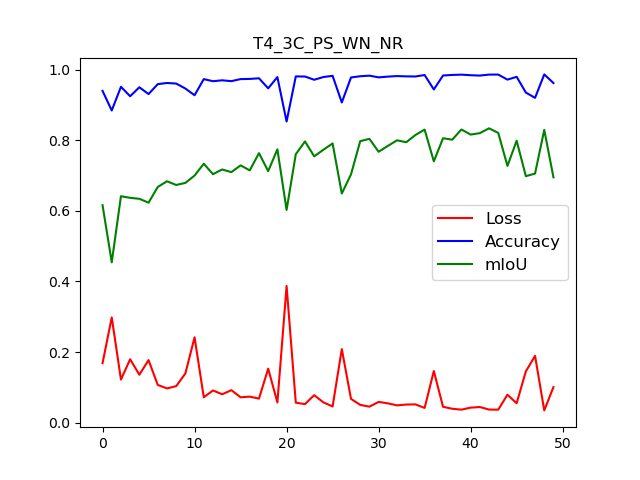
\includegraphics{./Images/T4_3C_PS_WN_NR.png}
    \caption{PointNet++ Trainings-Ergebnisse pro Epoche mit 3 Klassen und Normalisierung ohne zufällige Rotationen}
\end{figure}


Vergleich Training mit/ohne Normalen

Vergleich Training mit/ohne Normalisierung (Einsatz von nicht normalisierten Punkten trotz Normalisierung im Training möglich?)

Evaluations-Ergebnisse auf nicht normalisierten Daten für Training (t5) mit normalisiertem Datensatz:

eval mean loss: 0.174850

eval accuracy: 0.945604

eval avg class acc: 0.784519

eval mIoU of Plant:	 0.683556

eval mean mIoU: 0.683556

eval mean mIoU (all shapes): 0.683556

Evaluations-Ergebnisse auf normalisierten Daten für Training (t5) mit normalisiertem Datensatz:

eval mean loss: 0.038411

eval accuracy: 0.985966

eval avg class acc: 0.949488

eval mIoU of Plant:	 0.840759

eval mean mIoU: 0.840759

eval mean mIoU (all shapes): 0.840759

\begin{figure}
    \centering
        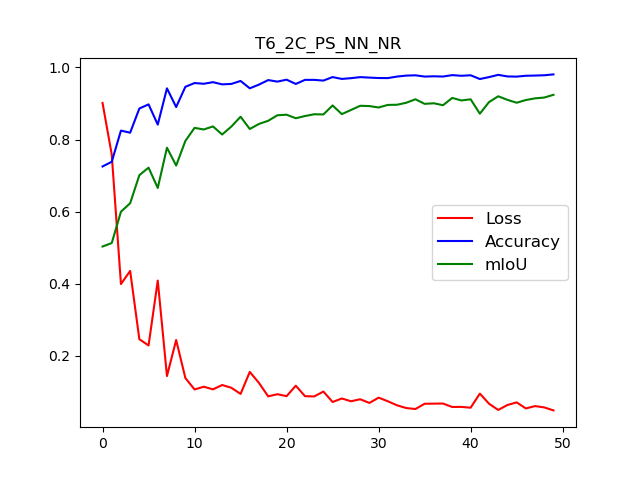
\includegraphics{./Images/T6_2C_PS_NN_NR.png}
    \caption{PointNet++ Trainings-Ergebnisse pro Epoche mit 2 Klassen, ohne Normalisierung und ohne zufällige Rotationen }
\end{figure}

\begin{figure}
    \centering
        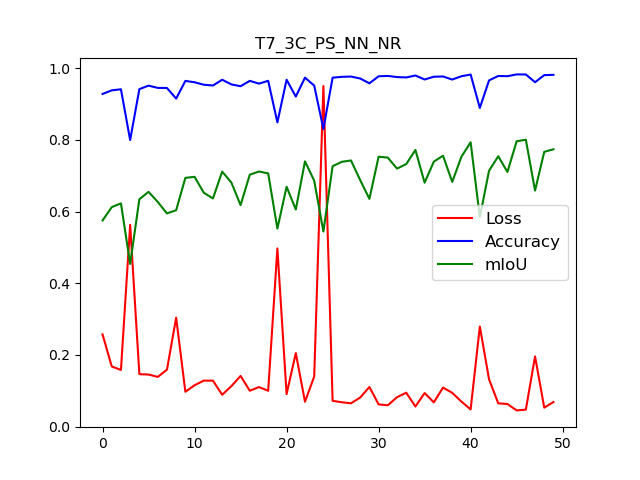
\includegraphics{./Images/T7_3C_PS_NN_NR.png}
    \caption{PointNet++ Trainings-Ergebnisse pro Epoche mit 3 Klassen, ohne Normalisierung und ohne zufällige Rotationen}
    \label{fig:T7_3C_PS_NN_NR}
\end{figure}

Die Tests des Servers haben gezeigt, das es bei der Segmentierung der freigestellten Pflanzen zu starken Fehlern kommt, wenn diese rotiert sind. 
Das hat zu der Erkenntnis geführt, dass PointNet++ anfällig für die Ausrichtung von Punktwolken ist. 
Aus diesem Grund wurde das Training für das zwei und drei Klassen-Netz mit zufälligen Rotationen wiederholt um ein Robustheit gegen Rotationen anzutrainieren.
Die Ergebnisse für zwei Klassen-Netz ist in Abbildung ~\ref{fig:10_2C_PS_WN_RR} zu sehen. Die Ergebnisse für das 3 Klassen-Netz in Abbildung ~\ref{fig:9_3C_PS_WN_RR}. 
Beim Training von dem Netz mit drei Klassen sind starke Ausreißer in den Loss-Werten zu erkennen die sich auch in der Accuracy und dem IoU wiederspiegeln.


\begin{figure}
    \centering
        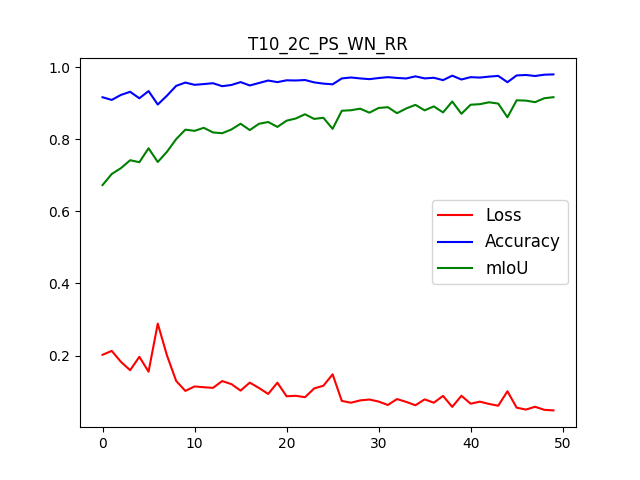
\includegraphics{./Images/10_2C_PS_WN_RR.png}
    \caption{PointNet++ Trainings-Ergebnisse pro Epoche mit 2 Klassen, mit Normalisierung und zufälliger Rotationen}
    \label{fig:10_2C_PS_WN_RR}
\end{figure}

\begin{figure}
    \centering
        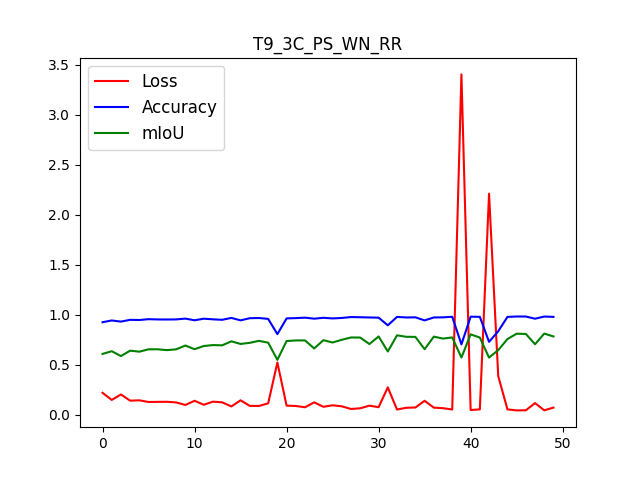
\includegraphics{./Images/9_3C_PS_WN_RR.png}
    \caption{PointNet++ Trainings-Ergebnisse pro Epoche mit 3 Klassen, mit Normalisierung und zufälliger Rotationen}
    \label{fig:9_3C_PS_WN_RR}
\end{figure}

\newpage
\section{Fazit und Ausblick}
%-------------------------------------------------------------
\label{sec:fazit}
%Am Ende der Arbeit muss ein Fazit dessen was geleistet wurde
%und wie es weitergehen kann. Dazu gehört auch wie der aktuelle
%Stand Ihrer Implementierung ist: ist Ihre Lösung z.B. bereits
%produktiv im Einsatz? Welche wesentlichen Punkte müssen noch
%umgesetzt werden?
%
%Insbesondere müssen hier die Schwachpunkte
%Ihrer Lösung erwähnt werden, also was Sie anders machen würden,
%wenn Sie dieselbe Aufgabe noch einmal bekämen. Auch nicht gelöste
%oder sich im Laufe der Arbeit neu ergebene Fragen müssen hier zur
%Sprache kommen.

Problem bei Registrierung mit unterschiedlich skalierten Punktwolken. Lösung Nutzung von GEO-Koordinaten bei der Generierung der Punktwolken oder ScaleLK?

%Weitere Analyse der Daten

\newpage
% Literaturverzeichnis
%-------------------------------------------------------------
\addcontentsline{toc}{section}{Literatur}
%\begin{thebibliography}{99}
%\raggedright
%\bibitem{buch} Autor(en): {\em Titel eines Buchs.}
%  Verlag, Auflage, Jahr
%\bibitem{artikel} Autor(en): {\em Überschrift eines Artikels.}
%  Zeitschriftennamen, Ausgabe, Seiten xx-yy, Jahr
%\bibitem{webseite} Autor(en): {\em Titel einer Webseite.}
%  \url{url}, Jahr/Datum der Erstellung\footnote{Nicht zitierfähige Webseiten sollten Sie nicht im Literaturverzeichnis auflisten, sondern als Fußnoten im laufenden Text als Quellen angeben.}
%\bibitem{opensource} Autor(en): {\em Name einer Software.}
%  Version, Datum, \url{url}
%\end{thebibliography}

\bibliographystyle{ieeetr}
\bibliography{./bibleografie.bib}

\end{document}